\documentclass[tikz,border=7pt]{standalone}
% end preamble
\usepackage[e]{esvect}
\usetikzlibrary{calc, angles}
\tikzset{
  line/.style = {
    shorten <=-3mm, shorten >=-3mm
  },
  vector/.style = {
    thick,-latex
  },
  dot/.style = {
    insert path={
      node[scale=2]{.}
    }
  },
  perp/.style = {draw,angle eccentricity=.5, angle radius=2mm,pic text=.},
}
\begin{document}
  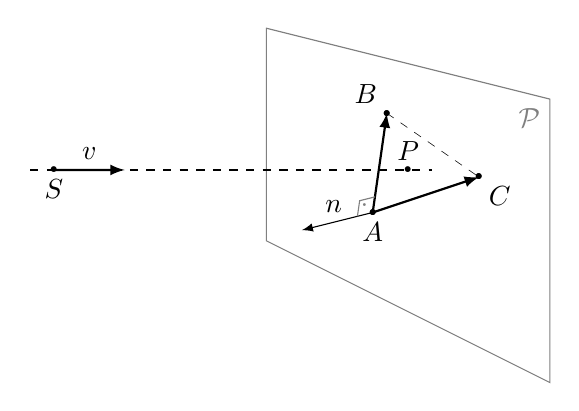
\begin{tikzpicture}[scale=0.9]
    % le plan
    \draw[gray]
      (0,0) coordinate (P1)
      -- ++(0,3) coordinate (P2)
      -- ++(4,-1) coordinate (P3)
      -- ++(0,-4) coordinate (P4)
      -- cycle
      (P3) node[below left]{$\mathcal{P}$}
    ;
    % les points A,B,C
    \path
      (1.5,.4) coordinate[label={center,scale=2:.}] (A)
      +(.2,1.4) coordinate[label={center,scale=2:.}] (B)
      +(1.5,.5) coordinate[label={center,scale=2:.}] (C)
    ;
    \draw
      (B) edge[very thin, dashed] (C)
      (A) edge[vector] (B)
      (A) edge[vector] (C)
    ;
    % le vecteur normal
    \path
      (A) coordinate (N)
      +(-1,-.25) coordinate (Na)
      (B) coordinate (Nn)
      (N) edge[-latex] node[above, pos=.55]{$\vv{n}$} (Na)
      pic[perp,gray]{right angle=Nn--N--Na}
    ;
    % le rayon
    \path
      (-3,1) coordinate (S)
      (2,1) coordinate (P)
      ($(S)!1cm!(P)$) coordinate (v)
    ;
    \draw
      (S) edge[line, dashed] (P)
    ;
    \draw
      (S) edge[vector] node[above, sloped]{$\vv{v}$} (v)
    ;
    \path
      (S) [dot] node[below]{$S$}
      (P) [dot] node[above]{$P$}
      (A) [dot] node[below]{$A$}
      (B) [dot] node[above left]{$B$}
      (C) [dot] node[below right]{$C$}
    ;
  \end{tikzpicture}
\end{document}
